\chapter{Radio Driver for Zolertia with the RN2483 module\label{section:radio}}

% Most of the LoRaWAN features were not implemented or tested since this was out of the scope of this project.

The \emph{Zolertia RE-Mote REV-B} platform does not support \emph{LoRa} out of
the box. This chapter covers the implementation of a radio driver on
\emph{Contiki-NG} for the \emph{RN2483}, a LoRa module from Microhip,
communicating with the \emph{RE-Mote} platform.

\section{Preliminary work}

Last year \emph{Roald Van Glabbeek}, in the course of his master thesis~\cite{8847137}, 
aiming at doing further research on \emph{energy efficient lora multihop networks}, 
started working on the \emph{RN2483} module.
For this purpose he made \emph{RN2483 Shields} adapted to the pin
configuration of the \emph{Zolertia RE-Mote REV-B}. He also started a radio driver
implementation for Contiki-OS\@.

In the previous attempt to adapt \emph{TSCH} for \emph{LoRa}
in~\cite{njomgang_2018}, Serge did his experimentation with the \emph{LoRaMote}
demo platform from \emph{Semtech} using a different LoRa radio module the
\emph{SX1272}. 
As analyzed in~\cite{8847137}, LoRaMotes turned out to be an issue for the
further research because they were no longer produced, 
new versions were expensive and memory was a bottleneck.
That is why the \emph{Zolertia RE-Mote} was chosen instead. 
The platform is already available 
and well maintained in \emph{contiki-ng} (making the transition faster and less
error prone as less code need to be developed) and the \emph{ETRO Lab} is
already using the platform.

The first part of my work consisted in implementing a reliable
and fully featured radio driver for the \emph{RN2483} module working in the last
version of \emph{contiki-ng}.

\section{RN2483 Module Structure}

Developed by \emph{Microchip} the \emph{RN2483} is a LoRa module operating in
the 433 MHz and 868 MHz Frequency Bands~\cite{microchip:rn2483}. 
The module is specifically designed to work with LoRaWAN compatible networks, 
by including a set of commands designed for seamless integration with the
\emph{LoRaWAN Protocol Stack}

Each communication to and from the module is done via \emph{UART} ASCII command,
making it easy for a human to interact with the module by handwriting commands
on a terminal and reading the response back in a readable format
(see~\ref{fig:pcconn}).
% The module is made for ease of use over performance and power consumption.

\begin{figure}[H] % TODO More info on axis
\centering
\begin{tikzpicture}[auto, thick]
  \node(pc) [server, label=below:{PC}] {};
  \node(ftdi) [draw, rectangle, right=of pc, right=4cm] {USB to UART Adapter};
  \node(module) [draw, rectangle, minimum size=6mm, right=of ftdi, right=2.5cm] (module) {RN2483 Module};

  \path (pc) edge[<->] node[]{USB Connection} (ftdi) ;
  \path (ftdi) edge[->,bend left] node[text width=1cm, align=center]{TX} (module);
  \path (module) edge[->,bend left] node[text width=1cm, align=center]{RX} (ftdi);
\end{tikzpicture}
\caption{Simple communication with the module scenario\label{fig:pcconn}}
\end{figure}


The module's interface includes three types of commands that enable access to
different functions~\cite{microchip:reference}.

\begin{itemize}
  \item \emph{radio} for the low-level radio commands to access the transceiver
    and PHY settings directly without the LoRaWAN interface overhead.
  \item \emph{mac} to access the LoRaWAN protocol stack configurations and
    commands. This command set will be used less because our implementation
    requires low-level transceiver access.
  \item \emph{sys} for the module specific configurations such as the module
    GPIOs state, \emph{sleep}, EEPROM memory access, \ldots
\end{itemize}

\section{Testing Setup}

My testing setup was the same as~\cite{8847137}. I used the Zolertia RE-Mote
Rev-B platform, using the CC2538 microcontroller, connected to the
RN2483 breakout board, as schematized in Fig~\ref{fig:schemaconn}. 

The RE-Mote platform has two UART peripheral, the UART1 peripheral is used
to communicate with the module because the platform debugger use UART0.

The \lstinline{PD0} GPIO is wired to the reset pin to allow
software reset of the module as well as a push button in case of hard reset.

\begin{figure}[H]
  \centering
  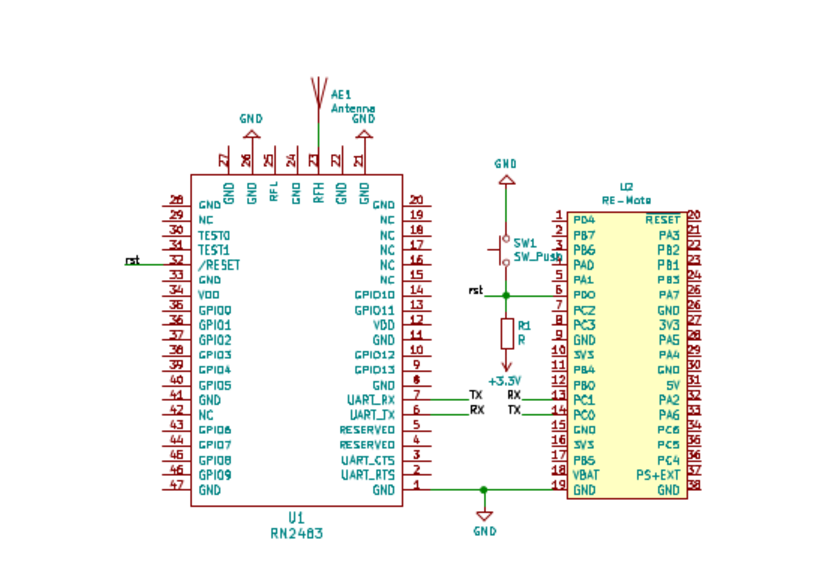
\includegraphics[scale=0.70]{thesis.tex/chapters/driver/fig/conn_diag.pdf}
  \caption{Hardware connection\label{fig:schemaconn}}
\end{figure}

\section{Implementation}

All the files for the driver implementation are available in
\lstinline{/arch/dev/rn2483} and the location of the examples are in
\lstinline{/examples/platform-specific/rn2483}.

\subsection{Structure}

My implementation structure took inspiration from the work 
in~\cite{8847137} and the \emph{RIOT-OS}
project\footnote{\url{https://github.com/RIOT-OS/RIOT}}. 

Following, is a listing of the different files I created and their
usage. % \improvement{I don't like this phrase}

\begin{description}
  \item[lora] LoRa radio specific functions declaration, and configuration. 
    This includes functions used to calculate the time on air and
    LoRa PHY configuration structure and parameters.
  \item[rn2483-include] contains the declaration both needed by
    \lstinline{rn2483-uart} and \lstinline{rn2483} to avoid cycling inclusion
    that mess with the compiler.
  \item[rn2483-uart] Lower level implementation of the function to directly
    communicate with the module via UART\@.
    It contains hardware specific implementation for the UART\@.
  \item[rn2483-api] Complete coverage of the RN2483 commands. Using functions
    from this file allow the user of the driver to not write
    each command by hand and use standard structure instead.
  \item[rn2483] Implementation of the Contiki radio device driver. 
    It contains the standardized way of Contiki to use and configure radio
    devices.
    All the radio driver in Contiki share this structure.
\end{description}

\subsection{Synchronous communication with the module}

The first design challenge is the
synchronous UART message mechanism implementation.
UART communication needs synchronous messaging for every
transmission, configuration, and reception.
Acknowledgements from commands avoid 
clashes when trying to use the module at the same time.
The previous implementation in~\cite{8847137} used fixed time delays to 
wait for the command to full execution on the module. This method 
quickly showed its own limitation, each command has their own delay and
fixed delays slow the global execution.

% TODO Maybe sequence diagram with a clash

My implementation of the UART driver for the CC2538 in Contiki does not have synchronous 
blocking read function out of the box, it assumes the programmer will compute the
responses from UART in processes waiting for an event instead.
Reception works by executing an \emph{input handler} at each interruption
triggered from UART reception.
Contiki set the default input handler with the function
\lstinline{serial_line_input_byte},
specifically designed for serial communication with terminals. 
I keep using this handler with UART0 to get debug messages from USB connections.

We have to define our own handler, for the UART1 peripheral, similarly as the
default one because they both use same message structure terminating by
\lstinline{\r\n}.
The function \lstinline{serial_line_input_byte} pass each character to standalone
process (\lstinline{serial_line_process}) and broadcast an event on command
full reception, instead our handler directly threat each message in an
interrupt.

Working with processes and events, is impossible in our use case because Contiki 
does not have any mechanisms that allows programmers to wait for an event inside a 
function and only allows it inside processes.
Doing everything inside a process is not an option for this project.
The custom handler is designed as a state machine (Fig~\ref{fig:cmdstate}) and 
works with its own reception buffer. It takes advantage of the limited response 
format from the RN2483 module to sort each new communication.

\begin{itemize}
  \item Asynchronous LoRa radio messages start with \lstinline{radio rx  }.
  \item \lstinline{radio_tx_ok} indicates the end of the radio transmission. 
  \item \lstinline{ok} indicate the acknowledgement of a command.
\end{itemize}

% Talk about the state machine

I implemented helper functions, to ease the command transmission and
acknowledgement between the RE-Mote and the RN2483.

\begin{description}
  \item[rn2483\_receive\_synch] busywait on the command states
    (Fig~\ref{fig:cmdstate}) until reaching the \emph{received} state, 
    or the timeout duration has elapsed.
  \item[rn2483\_send\_cmd] a \emph{printf} style command, automatically 
    waiting for the acknowledgement (with the possibility to add custom timeouts).
  \item[rn2483\_raw\_cmd] sending the command from a buffer in argument
    without formatting or waiting for the acknowledgement.
\end{description}

\begin{figure}[H]
\centering
  \begin{tikzpicture}[->,>=stealth',shorten >=1pt,auto,node distance=3.5cm]
  \tikzstyle{every state}=[thick,draw=gray!50,fill=gray!20,draw=none,text=black]

  \node[initial,state] (A)                    {Transmission};
  \node[state]         (B) [above right of=A] {Reception};
  \node[state]         (C) [below of=B]       {Timeout};
  \node[state]         (D) [right of=B]       {Received};

  \path (A) edge [bend right]    node {     } (B)
            edge [bend left]     node {     } (C)
        (B) edge [bend left]     node {     } (C)
            edge                 node {     } (D)
        (C) edge [bend left]     node {     } (A)
        (D) edge [bend right=85] node {     } (A);
\end{tikzpicture}
\caption{The command states\label{fig:cmdstate}}
\end{figure}


\subsection{Transmission}

The radio transmission command has a different pattern from the other commands 
of the module. 
After the acknowledgement of the radio transmission command (\lstinline{radio tx ...}),
the module transmits a second message when the radio communication is done.

\begin{figure}[H]
\centering

\begin{sequencediagram}

\newthread{A}{RE-Mote}{}
\newinst[1]{B}{RN2483}{}
\newinst[3]{C}{Radio Band}{}
\begin{call}{A}{radio tx~\ldots}{B}{radio\_tx\_ok}
  \messdash{B}{ok}{A}
  
  \begin{sdblock}{Radio Transmission}{Transmition time calculated
    in~\ref{eq:tpacket}}
    \begin{call}[4]{B}{}{C}{}
    \end{call}
  \end{sdblock}
\end{call}

\end{sequencediagram}

  \caption{\lstinline{radio tx} command sequence diagram\label{fig:txsequence}}

\end{figure}



Microchip choses to represent the payload as string formatted hex number to
facilitate the manual writing of commands, making the message payload twice as
long as its original content. 
As all the content we will handle is represented as an \emph{8 bit} number array, 
I took the function to convert array to string representation and vice versa
from the RIOT-OS project.
% TODO REF

\subsection{Asynchronous Reception}

The last component of a complete driver implementation is to receive radio
messages.
Reception follows a different scheme from the other commands. 
New message reception can happen at any time, asynchronously, from the moment
we run the command \lstinline{radio rx 0}.
I implemented a one message inbox to tackle this issue (see Fig~\ref{fig:rxstate}).

Every message coming from the module is analyzed.
Radio communication, starting with \lstinline{radio rx }, set a flag to indicate the 
presence of a new message. 
This flag remains until the message is read with the driver.
Messages are received in a string formatted hex number, that we must convert it to an
\emph{8 bit integer array}. 
% TODO Talk about packet buf ?
% We don't store the final result in the same buffer as the one used for
% reception as reading the result 
% This array is stored in a different place than the received message as command
% may be executed between the moment we receive the message and the moment we
% read it.
Also, a timestamp is saved at the reception to keep track of when the
message was received.

\begin{figure}[H]
\centering
  \begin{tikzpicture}[->,>=stealth',shorten >=1pt,auto,node distance=3.5cm]
  \tikzstyle{every state}=[thick,draw=gray!50,fill=gray!20,draw=none,text=black]

  \node[initial,state] (A)              {None};
  \node[state]         (B) [right of=A] {Received};

    \path (A) edge [bend right] node[below] {Reception} (B)
          (B) edge [bend right] node[above] {Read} (A);
\end{tikzpicture}
\caption{The RX states\label{fig:rxstate}}
\end{figure}


\subsection{Contiki Radio Driver}

The Contiki WIKI did not provide any information about writing our own radio driver
or porting a new radio platform for Contiki.
I based my implementation on the other radio driver implementation already
available on Contiki to understand the driver structure.

To create a Contiki radio driver we have to implement a \lstinline{radio_driver}
structure that must implement the following functions.

\begin{description}
  \item[init] is the first function of the driver executed at startup.
    The configuration of the RN2483 into point-to-point mode takes place here.
  \item[prepare] is the function called before a transmission with the data we
    want to transmit as parameter. 
    We can not transmit radio messages while listening for incoming messages, the
    first step of preparation is to exit the radio reception mode with the
    command \lstinline{radio rxstop}.
    The function take care to convert the data in the command ready to be sent.
  \item[transmit] sends the already formatted command in the prepare function and
    waits for the \lstinline{radio_tx_ok} acknowledgement.
  \item[send] is the combination of prepare and transmit.
  \item[read], on radio message reception, the function copies the 
    message to the buffer passed in the argument.
  \item[channel\_clear]
  \item[receiving\_packet] should theoretically check if the radio module is
    currently getting a new message from a transmission. This is a function we
    can expect from some platforms with integrated radio module but here the
    simplicity of the RN2483 shows its limitations and I found no way for the module
    to acknowledge when it receiving a new message.
  \item[pending\_packet] checks the message inbox to see if we received a new
    message.
  \item[on] wake-up the module and starts listening to radio messages.
  \item[off] stop listening to radio messages and put the module to sleep.
  \item[get\_value, set\_value, get\_object, set\_object] are all the functions used
    to configure the radio driver for a different network layer. 
    The parameters we need to implement will be discussed in Chapter~\ref{section:tsch}.
\end{description}

% TODO talk about Poll mode

\section{Validation test}

To verify the implementation of the radio driver two examples are available.

\begin{itemize}
  \item The \emph{RN2483 shell} available in
    \lstinline{/example/platform-specific/lora/rn2483} is a tool to interact
    directly with the module.
  \item The \emph{ping-pong} example based on the nullnet example already
    available in \emph{contiki-ng} located in 
    \lstinline{/example/platform-specific/lora/nullnet} demonstrate the driver
    is correctly working with upper layer of the network stack.
\end{itemize}

% For each Contiki project, \emph{Contiki's Network Protocol stack}, also known
% as \lstinline{NETSTACK}, defines the different OSI layers implementations we 
% want to use in our project (Fig~\ref{fig:netstack}).
Each project is bundled with a \lstinline{project-conf.h}
configuration file in which we can define the parameters of our project. 
To set my LoRa driver as the physical layer implementation we must add the
following line to change the NETSTACK configuration.

\begin{lstlisting}
#define NETSTACK_CONF_RADIO rn2483_radio_driver
\end{lstlisting}

\subsection{Shell}

This example extends the existing shell available in Contiki by writing a set
of commands to test and interact with the RN2483 via UART\@.

Here is the list of the added commands to the Contiki shell.

\begin{lstlisting}[language=none]
'> sys': Send a 'system' command to the RN2483 Module.
'> mac': Send a 'mac' command to the RN2483 Module.
'> radio': Send a 'radio' command to the RN2483 Module.
'> tx': Transmit a radio message with the RN2483.
'> sleep': Put RN2483 into sleep mode.
'> wakeup': Force wakeup of RN2483.
'> rn2483_reset': Hardware Reset of the RN2483 Module.
'> help': Shows this help.
\end{lstlisting}

This was used during the development of the driver as a way to test parameters
as well as the synchronous communication implementation.

\subsection{Ping-Pong\label{section:pingpong}}

I based this example on the \emph{nullnet-broadcast} example to test if two
nodes could communicate using the LoRa driver I implemented when controlled by
the \emph{CSMA} MAC layer instead of directly using the driver API\@.

The example is using the NETSTACK in Fig~\ref{fig:pingpongstack}.

\begin{figure}[H]
\centering
  \begin{tikzpicture}[->,>=stealth',shorten >=1pt,auto,node distance=1.6cm]

  \tikzstyle{comment}=[
    right=2pt,
    font=\small,
    fill=white,
    text=black,
    draw=black,
  ]

  \tikzstyle{every state}=[rectangle,thick,
    draw=black,fill=gray!20,text=black,
    minimum width= 6cm,
    minimum height= 1.20cm
  ]

  \tikzstyle{smallstate}=[rectangle,thick,
    draw=black,fill=gray!10,text=black,
    minimum width= 4cm,
    minimum height= 1.20cm
  ]

  \node[smallstate]         (A)                    {Null Net};
  \node[smallstate]         (B) [below of=A]       {Null Routing};
\begin{scope}[on background layer]
  \node[state, fit=(A)(B)] (AB)                 {};
\end{scope}
  \node[state,below=1cm]         (C) [below of=AB]       {CSMA};
  \node[state]         (D) [below of=C]       {LoRa};

  \node[comment]       at (AB.north west) {Network Layer};
  \node[comment]       at (C.north west) {MAC Layer};
  \node[comment]       at (D.north west) {Physical Layer};
  % \path (A) edge [bend right]    node {     } (B)
  %           edge [bend left]     node {     } (C)
  %       (B) edge [bend left]     node {     } (C)
  %           edge                 node {     } (D)
  %       (C) edge [bend left]     node {     } (A)
  %       (D) edge [bend right=85] node {     } (A);
\end{tikzpicture}
\caption{The network stack used for the ping-pong example\label{fig:pingpongstack}}
\end{figure}


The example is a simple two-way communication between two RE-Motes. 
The first one is sending a request with a number as
payload and wait for the acknowledgement from the second motes sending back
the same payload. 
No other request is sent until the acknowledgement is received.
This is schematized in Fig~\ref{fig:pingpongsequence}.

The two different implementations to upload on two nodes are available in the
example folder.

\begin{itemize}
  \item \lstinline{ping.c} send the request and wait for an acknowledgement.
  \item \lstinline{pong.c} send the acknowledgement.
\end{itemize}

\begin{figure}[H]
\centering

\begin{sequencediagram}

\newthread{A}{Mote A}{}
\newinst[1]{B}{Mote B}{}

\begin{call}[4]{A}{ping}{B}{pong}
\end{call}
\end{sequencediagram}

\caption{Description of the execution of the ping-pong example\label{fig:pingpongsequence}}

\end{figure}


